% Раздел 3.4: Модуль «Регистрация и вход»
\subsection{Модуль «Регистрация и вход»}

В системе предусмотрены три сценария регистрации: для университета, студентов и преподавателей. В URL-параметрах передаются данные приглашения для последующей валидации и передачи на сервер.

Выбор формы регистрации осуществляется в зависимости от типа пользователя, переданного через параметры URL-строки. Пример логики выбора виджета приведён в листинге~\ref{lst:registration_widget_select}.

\begin{lstlisting}[caption={Выбор виджета регистрации по типу}, label={lst:registration_widget_select}]
const getForm = () => {
    const type = getSearchParams(REGISTRATION_TYPE_PARAM_NAME) as RegistrationTypesType;
    const inviteId = getInviteId();
    switch (type) {
        case 'teacher':
            return <RegistrationTeacherWidget inviteId={inviteId} />;
        case 'student':
            return <RegistrationStudentWidget inviteId={inviteId} />;
        case 'university':
        default:
            return <RegistrationUniversityWidget />;
    }
};
\end{lstlisting}
На рисунке~\ref{fig:registration_university} показан интерфейс страницы регистрации университета. Пользователь должен ввести название учебного заведения, фамилию, имя и отчество контактного лица, почты администрации университета, а также задать и подтвердить пароль. После заполнения всех обязательных полей и нажатия кнопки «Зарегистрировать университет» инициируется отправка данных на сервер.

\begin{figure}[h]
    \centering
    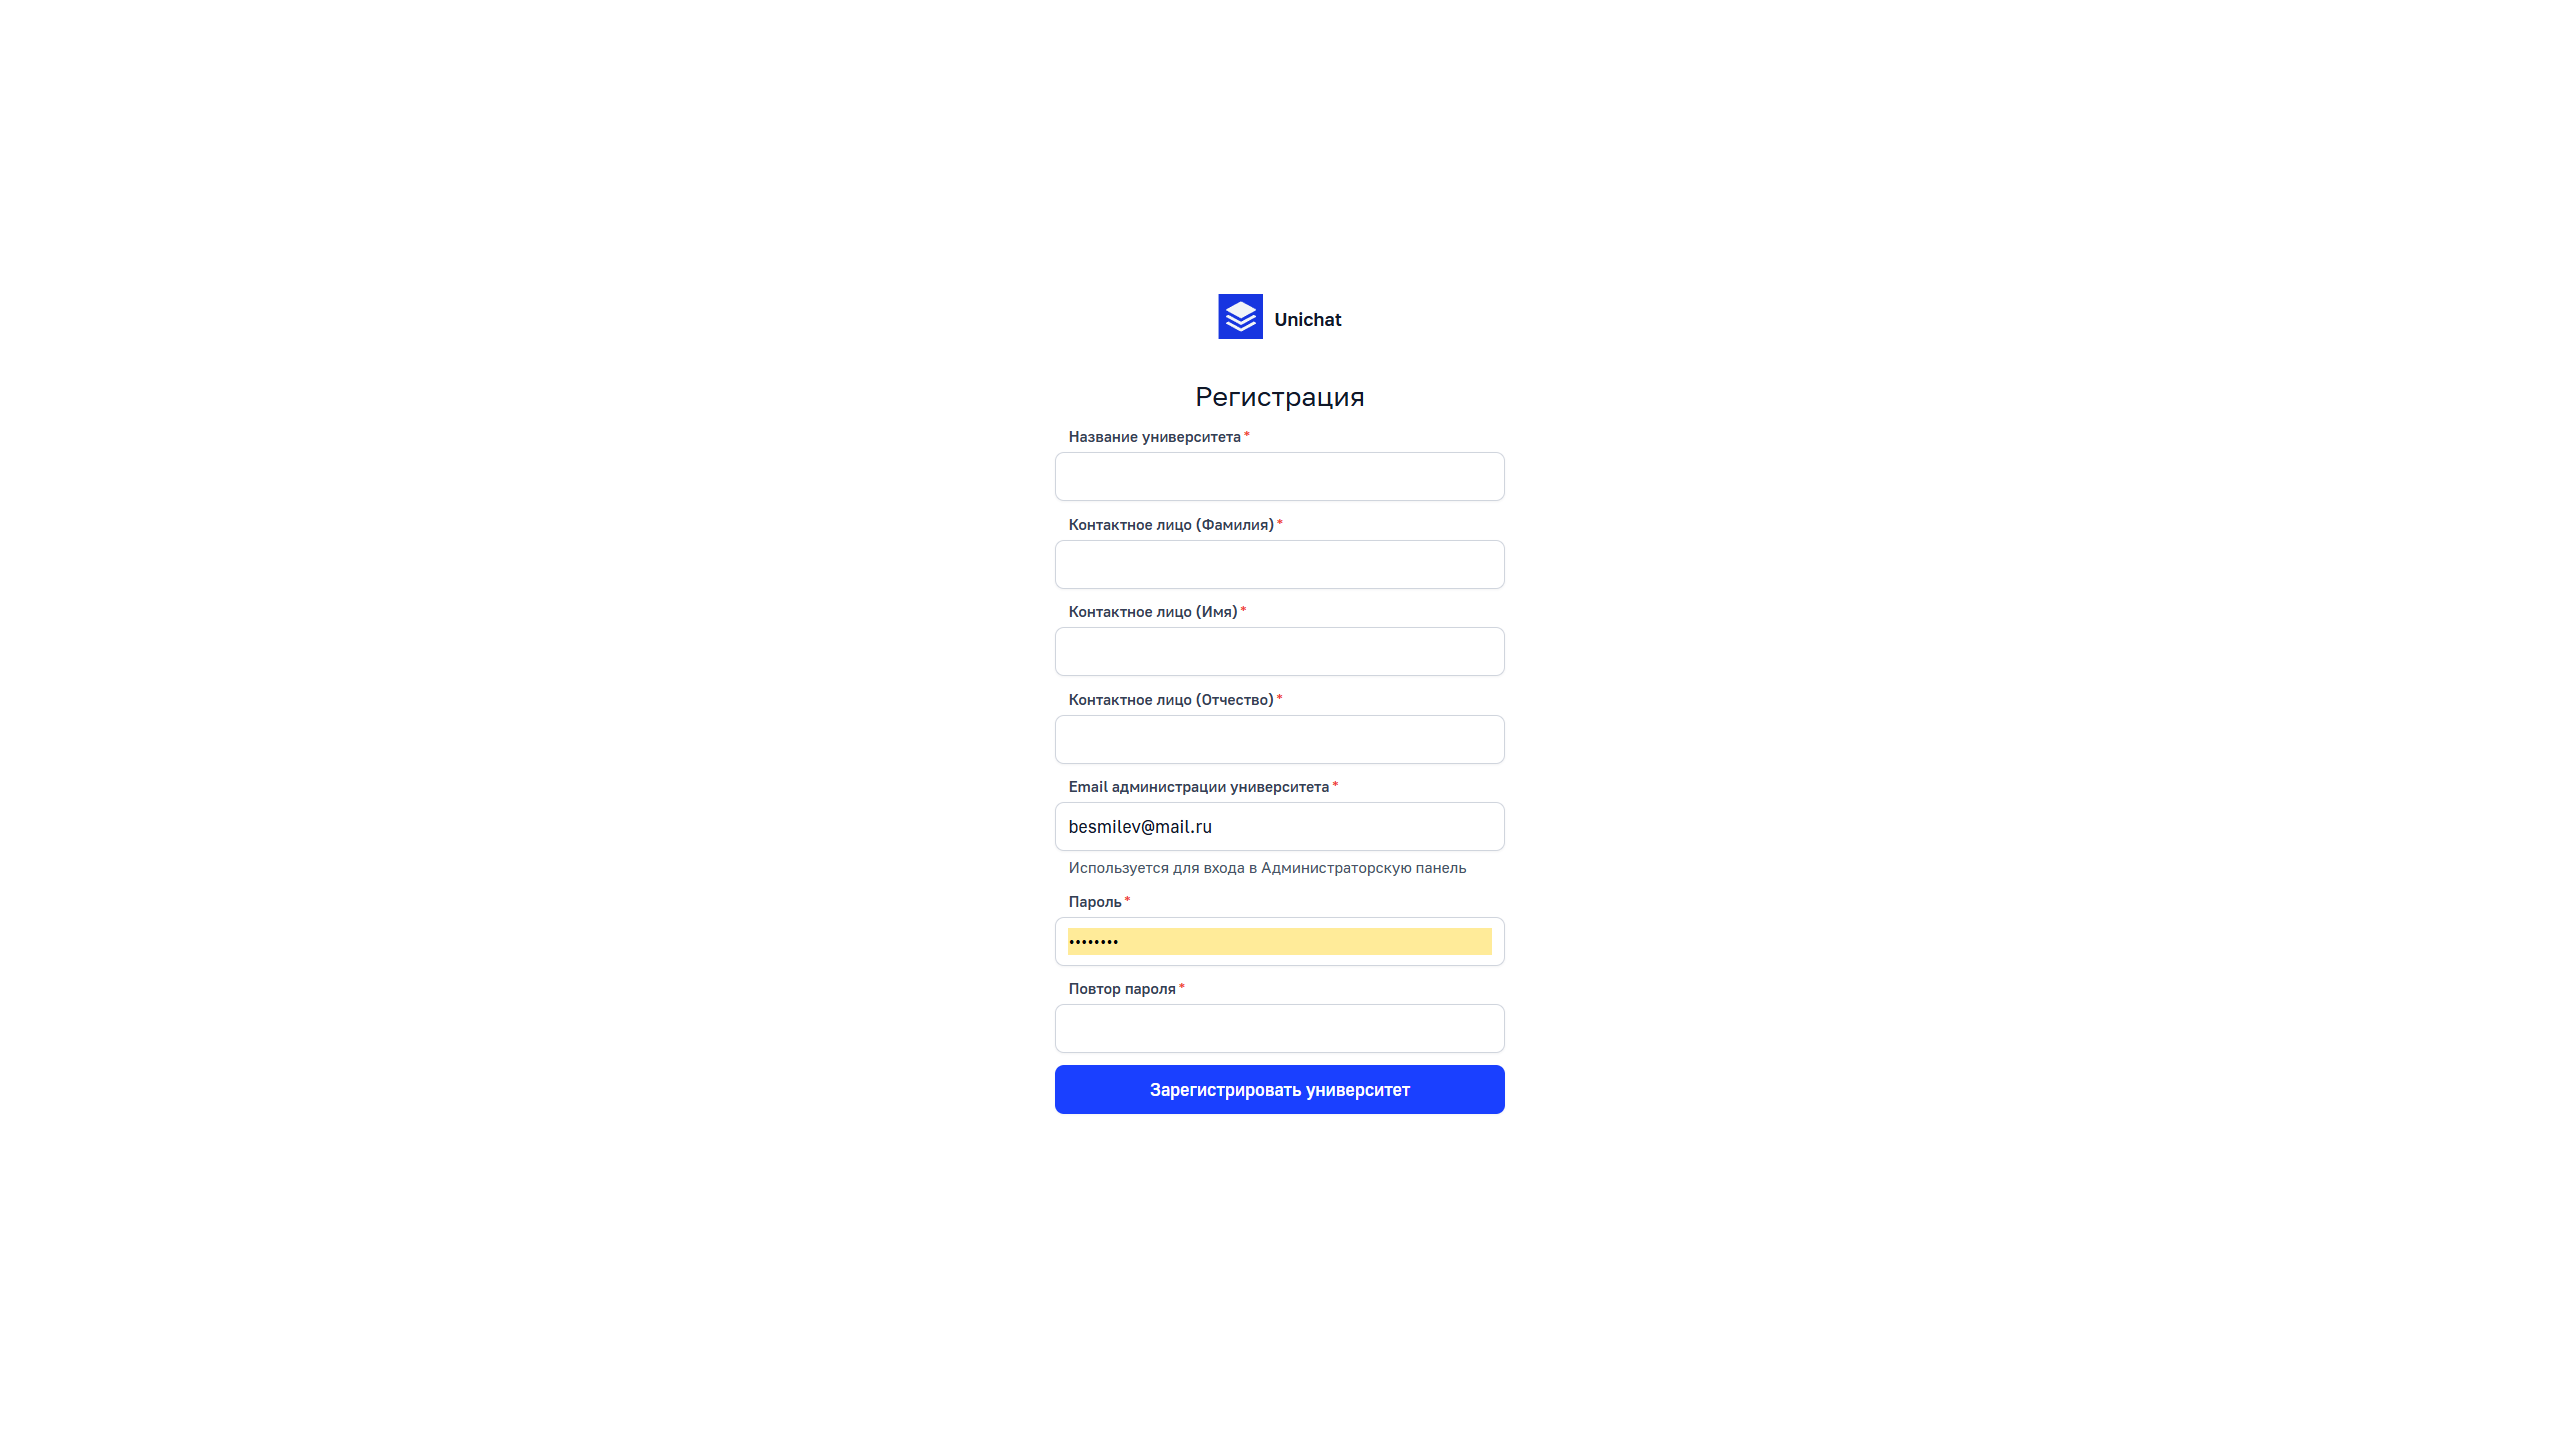
\includegraphics[width=0.5\textwidth]{static/presintation/RegPage.png} % Путь фейковый, замените на реальный при компиляции
    \caption{Страница регистрации университета: поля для названия института, контактного лица (ФИО), почты администрации, пароля и подтверждения пароля.}
    \label{fig:registration_university}
\end{figure}

Листинг~\ref{lst:registration_teacher_widget} демонстрирует структуру виджета регистрации преподавателя. Здесь реализована обработка валидности приглашения и логика отображения состояния формы в зависимости от результата асинхронной проверки.

\begin{lstlisting}[caption={Виджет регистрации преподавателя}, label={lst:registration_teacher_widget}]
export function RegistrationTeacherWidget({ inviteId }: RegistrationPropsType) {
    const { initData, onSubmit, isError, setIsError, formDataRef } =
        useRegistrationStudentAndTeacher<typeof registerTeacher>({
            inviteId,
            registrationRequest: registerTeacher
        });

    if (initData === undefined) {
        return 'Loading';
    }

    if (initData === null) {
        // Неверное приглашение или оно истекло
        return 'Error';
    }

    // Дальнейшая логика отображения формы регистрации преподавателя
    ...
}
\end{lstlisting}

\begin{figure}[h]
    \centering
    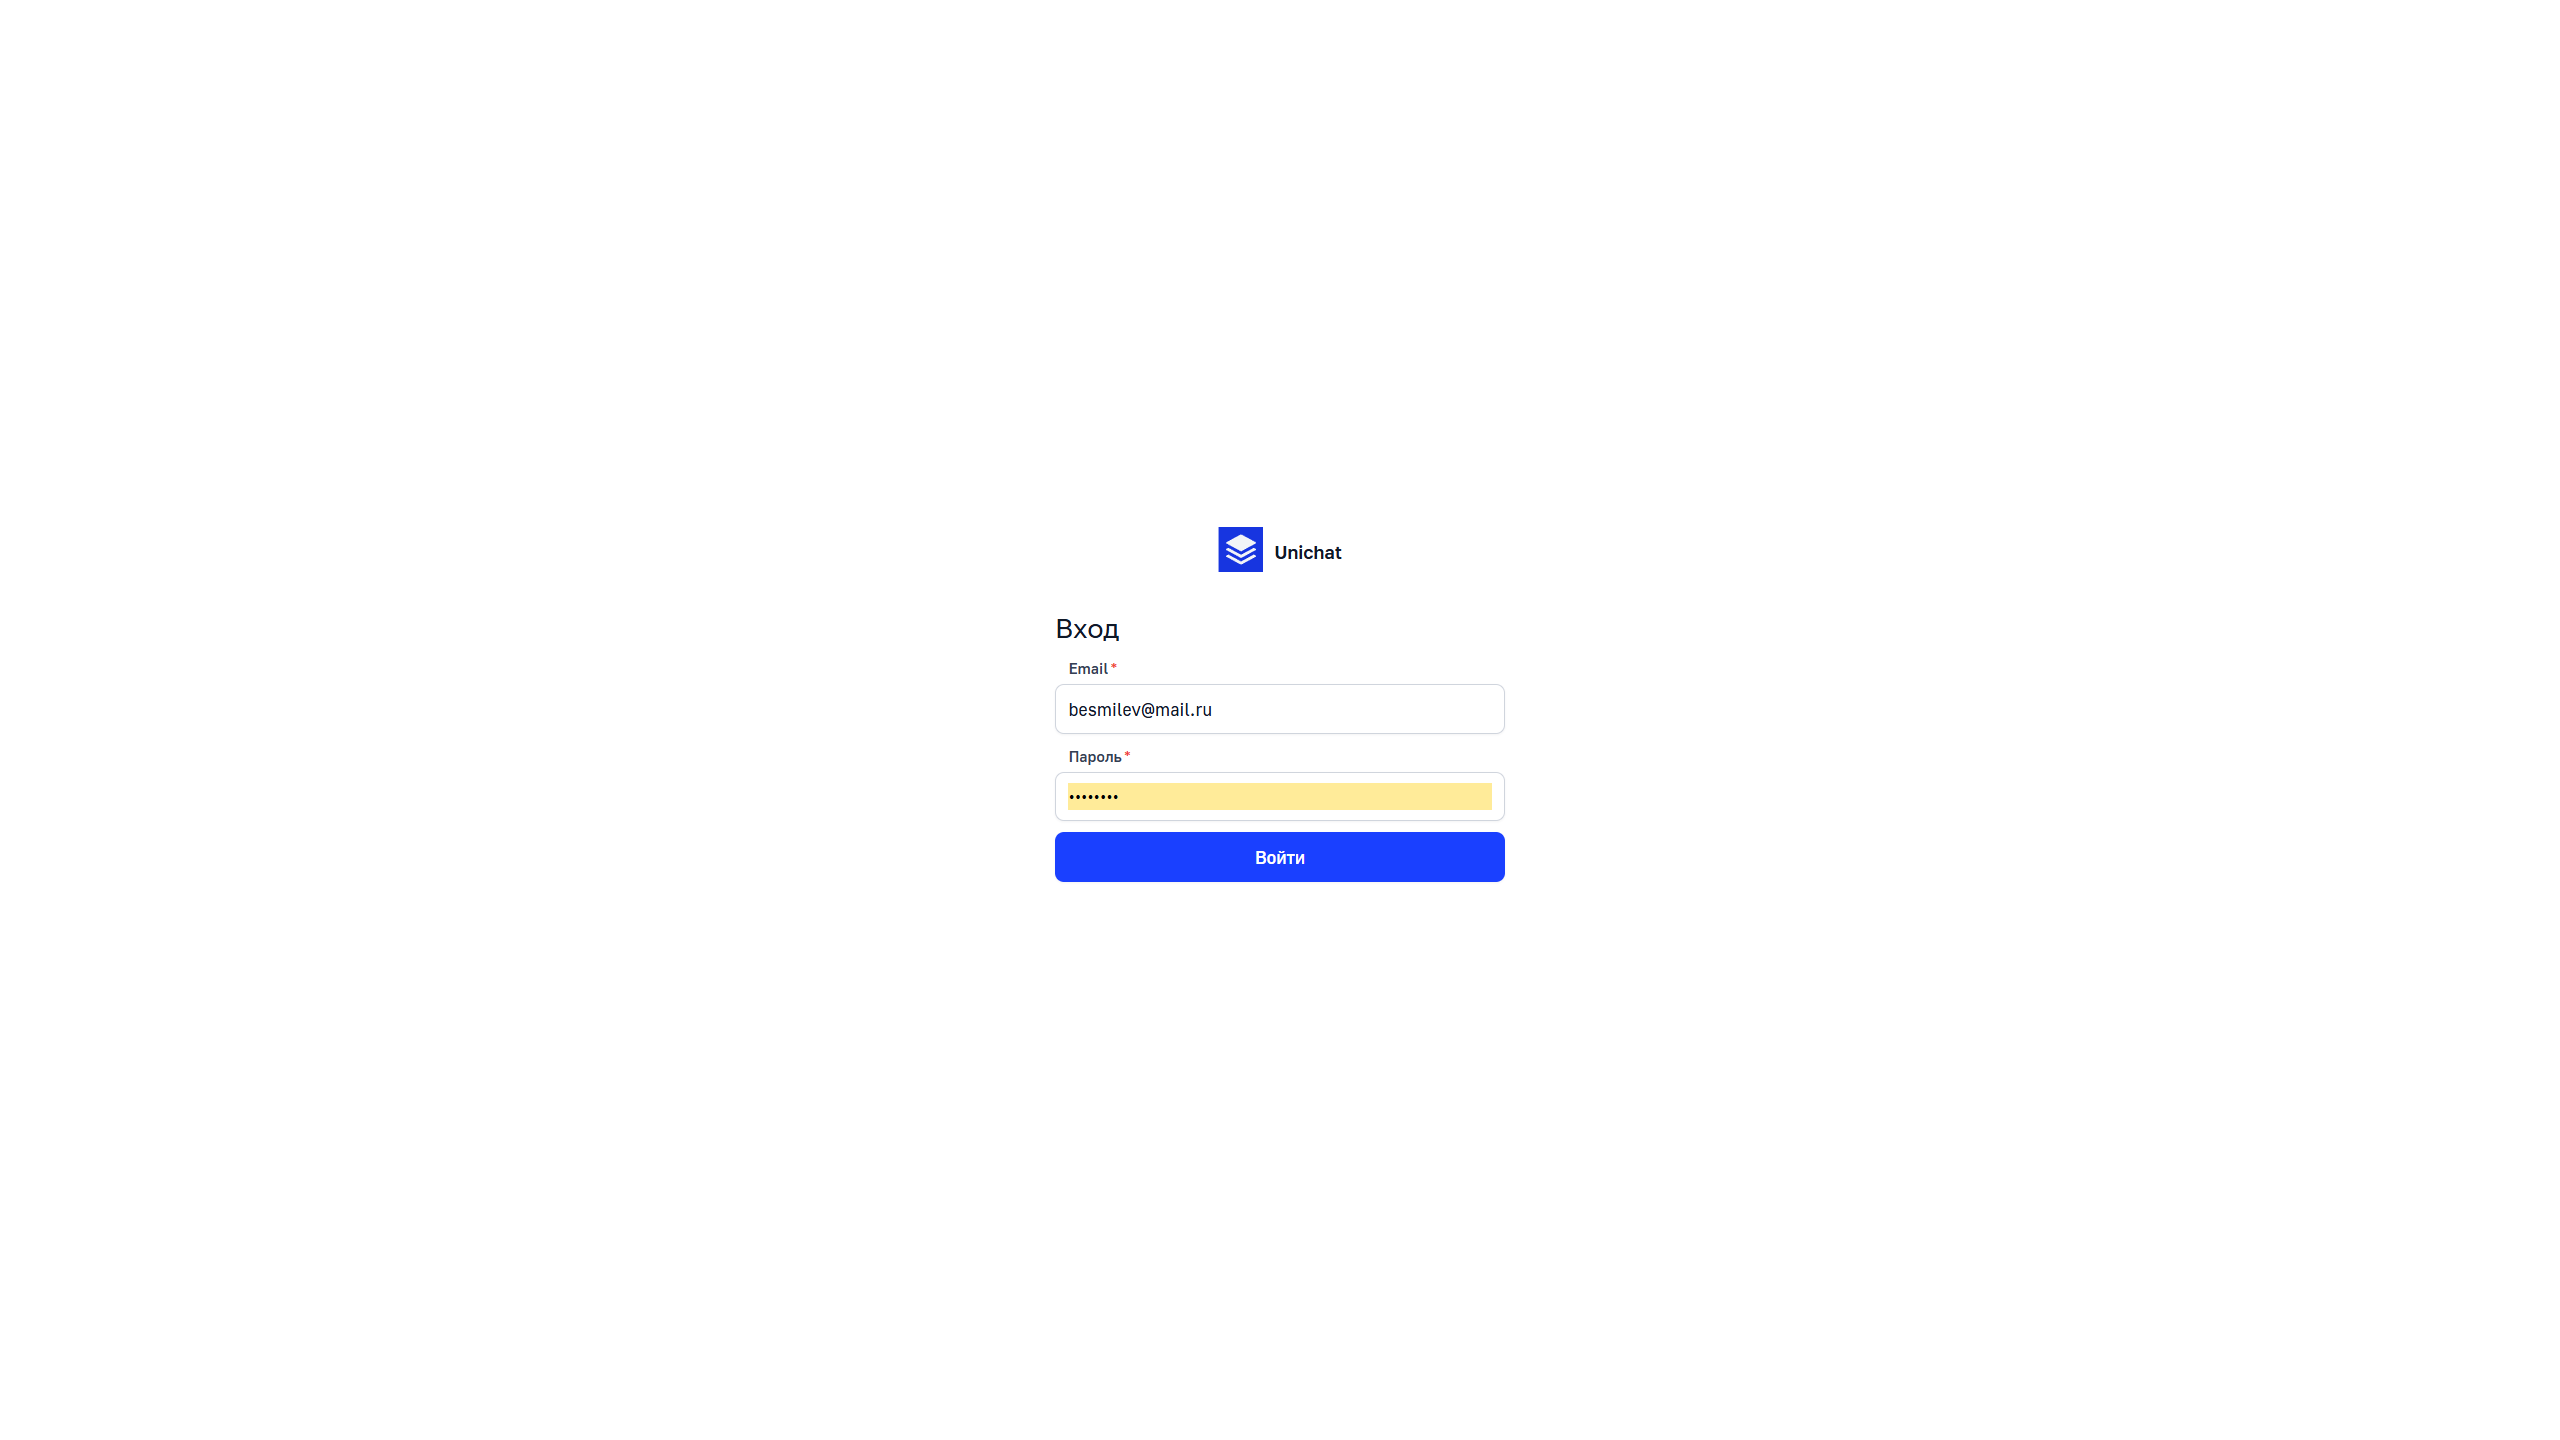
\includegraphics[width=0.5\textwidth]{static/presintation/LoginPage.png} % Путь фейковый, замените на реальный при компиляции
    \caption{Экран входа в систему: поля для ввода почты и пароля, а также кнопка «Войти».}
    \label{fig:login_page}
\end{figure}

На рисунке~\ref{fig:login_page} представлен экран входа в систему. Для авторизации пользователь вводит почту и пароль, после чего нажимает кнопку «Войти». В случае успешной авторизации система перенаправляет его в личный кабинет; при некорректных учётных данных отображается сообщение об ошибке.

% Конец раздела 3.4
